% Created 2024-01-28 Sun 19:42
% Intended LaTeX compiler: pdflatex
\documentclass[presentation]{beamer}
\usepackage[utf8]{inputenc}
\usepackage[T1]{fontenc}
\usepackage{graphicx}
\usepackage{longtable}
\usepackage{wrapfig}
\usepackage{rotating}
\usepackage[normalem]{ulem}
\usepackage{amsmath}
\usepackage{amssymb}
\usepackage{capt-of}
\usepackage{hyperref}
\mode<beamer>{\usetheme{Madrid}}
\definecolor{SUred}{rgb}{0.59375, 0, 0.17969} % SU red (primary)
\definecolor{SUblue}{rgb}{0, 0.17578, 0.38281} % SU blue (secondary)
\setbeamercolor{palette primary}{bg=SUred,fg=white}
\setbeamercolor{palette secondary}{bg=SUblue,fg=white}
\setbeamercolor{palette tertiary}{bg=SUblue,fg=white}
\setbeamercolor{palette quaternary}{bg=SUblue,fg=white}
\setbeamercolor{structure}{fg=SUblue} % itemize, enumerate, etc
\setbeamercolor{section in toc}{fg=SUblue} % TOC sections
% Override palette coloring with secondary
\setbeamercolor{subsection in head/foot}{bg=SUblue,fg=white}
\setbeamercolor{date in head/foot}{bg=SUblue,fg=white}
\institute[SU]{Shenandoah University}
\titlegraphic{
\includegraphics[width=0.5\textwidth]{\string~/Documents/suLogo/suLogo.pdf}}
\usetheme{default}
\author{Chase Mathison\thanks{cmathiso@su.edu}}
\date{29 January 2024}
\title{Area between curves}
\hypersetup{
 pdfauthor={Chase Mathison},
 pdftitle={Area between curves},
 pdfkeywords={},
 pdfsubject={},
 pdfcreator={Emacs 29.1 (Org mode 9.6.7)}, 
 pdflang={English}}
\begin{document}

\maketitle

\section{Announcements}
\label{sec:orgf77aaff}
\begin{frame}[label={sec:org8caf16e}]{Announcements}
\begin{enumerate}
\item Homework due tonight! in MyOpenMath!
\item Quiz on Friday.
\item Office hours: M - F, 10am - 11am.
\end{enumerate}
\end{frame}

\section{The lecture}
\label{sec:orgbe84ae6}
\begin{frame}[label={sec:org20d7997}]{Area between curves}
We know that we arrived at the definition of the definite integral by
considering the area under the curve given by \(y = f(x)\).  
We can use the definite integral to find more general areas.  For instance,
we can find the area bounded by the two curves
\[ y = x,\quad \text{ and } \quad y = x^2 \]
\begin{center}
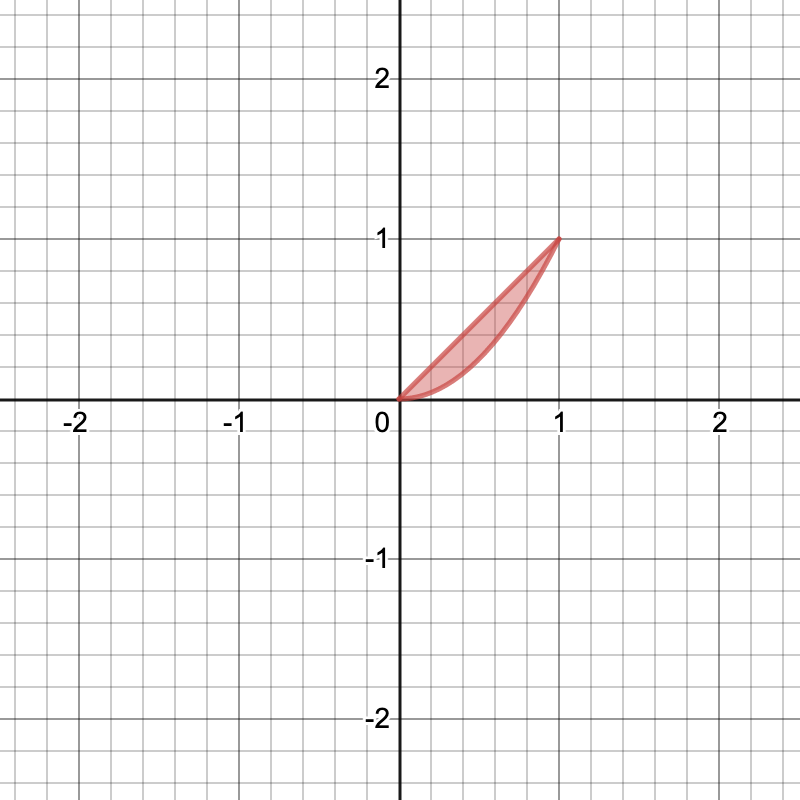
\includegraphics[width=0.3\textwidth]{../img/day004-ex1.png}
\end{center}
Let's see how!
\end{frame}

\begin{frame}[label={sec:orgaa3491a}]{Area between curves}
Assume for now that for \(a \le x \le b\) we have \(f(x) \ge g(x)\).  Then, to find the area between \(f(x)\) and \(g(x)\), let's
look at a sketch of what's going on:

\vspace{10in}
\end{frame}

\begin{frame}[label={sec:org6a417df}]{Area between curves}
\end{frame}

\begin{frame}[label={sec:orgb60e791}]{Area between curves}
The previous slides showed that if \(f(x) \ge g(x)\) for \(a \le x
\le b\), then the area between \(f(x)\) and \(g(x)\) is given by:
\vspace{10in}
\end{frame}

\begin{frame}[label={sec:orgee0ad1f}]{Example}
Find the area bounded by the graphs of the functions
\(f(x) = x\) and \(g(x) = x^4\).
\vspace{10in}
\end{frame}

\begin{frame}[label={sec:org16bbf68}]{Example}
\end{frame}

\begin{frame}[label={sec:org6cd989d}]{Example}
Let \(n > 0\).  Find the area bounded by the graphs of the functions
\(f(x) = x\) and \(g (x) = x^n\) with \(x \ge 0\).  What is the limit of this area as
\(n \rightarrow \infty\)?
\vspace{10in}
\end{frame}

\begin{frame}[label={sec:orgb3d7ca9}]{Example}
\end{frame}

\begin{frame}[label={sec:orgf775f96}]{When the curves switch}
We've only considered so far the area between two curves where one
function is always greater than the other function, but what about if
we want to find the area between two curves where the ``top curve''
switches?  Well, that's simply given by
\[
\int\limits_a^b \left| f(x) - g(x) \right|\,dx \]
\end{frame}

\begin{frame}[label={sec:org40dfd6f}]{Example}
Find the area between the curves
\[
f \left( x \right) = \sin \left( 2x \right) \quad \text{ and } \quad g
\left( x \right) = \cos \left( x \right)\]
between \(x = 0\) and \(x = \pi/2\).

\begin{center}
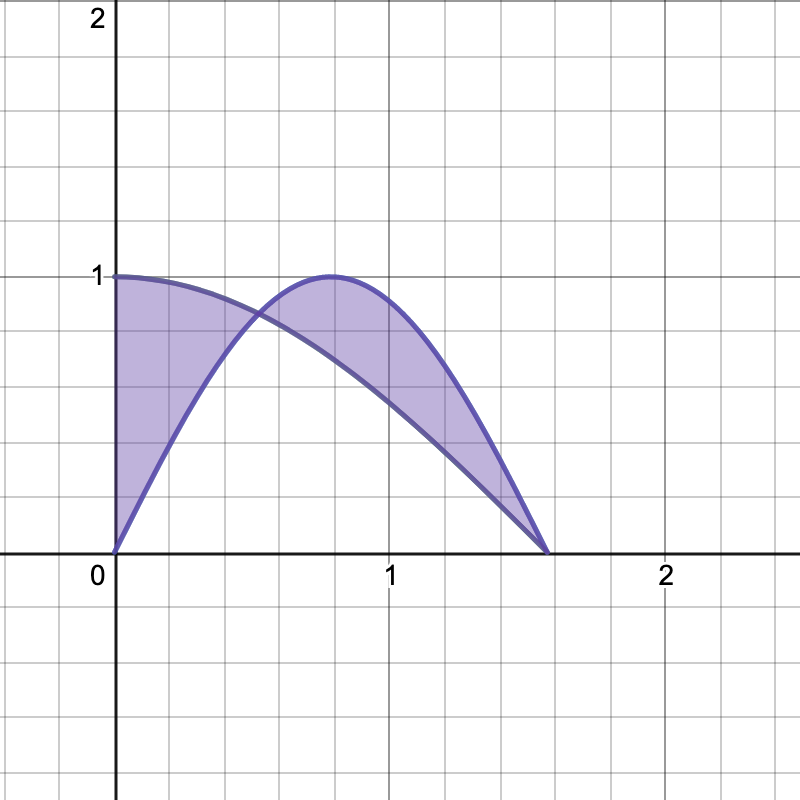
\includegraphics[width=0.4\textwidth]{../img/day004-ex2.png}
\end{center}
\end{frame}

\begin{frame}[label={sec:org23947ec}]{Example}
\end{frame}

\begin{frame}[label={sec:orgcc86c5c}]{A different example}
Let's consider finding the area bounded by the curves given by the
functions
\[
f(x) = x^2, \quad g(x) = 2 - x, \quad h(x) = 0 \]
for \(0 \le x \le 2\).
\begin{center}
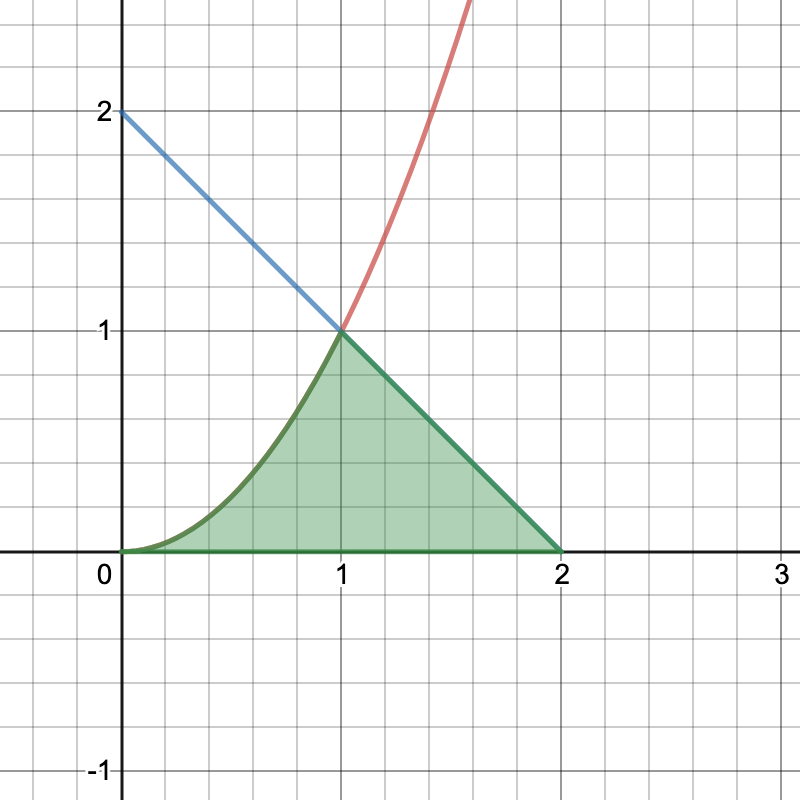
\includegraphics[width=0.4\textwidth]{../img/day004-ex3.png}
\end{center}
\end{frame}

\begin{frame}[label={sec:org0ebfc53}]{A different example}
\end{frame}

\begin{frame}[label={sec:org93662e0}]{Parting word}
We'll see a simpler way to tackle that last example in the next class.

Don't forget about homework!
\end{frame}
\end{document}